% Options for packages loaded elsewhere
\PassOptionsToPackage{unicode}{hyperref}
\PassOptionsToPackage{hyphens}{url}
\PassOptionsToPackage{dvipsnames,svgnames,x11names}{xcolor}
%
\documentclass[
  letterpaper,
  DIV=11,
  numbers=noendperiod]{scrartcl}

\usepackage{amsmath,amssymb}
\usepackage{iftex}
\ifPDFTeX
  \usepackage[T1]{fontenc}
  \usepackage[utf8]{inputenc}
  \usepackage{textcomp} % provide euro and other symbols
\else % if luatex or xetex
  \usepackage{unicode-math}
  \defaultfontfeatures{Scale=MatchLowercase}
  \defaultfontfeatures[\rmfamily]{Ligatures=TeX,Scale=1}
\fi
\usepackage{lmodern}
\ifPDFTeX\else  
    % xetex/luatex font selection
\fi
% Use upquote if available, for straight quotes in verbatim environments
\IfFileExists{upquote.sty}{\usepackage{upquote}}{}
\IfFileExists{microtype.sty}{% use microtype if available
  \usepackage[]{microtype}
  \UseMicrotypeSet[protrusion]{basicmath} % disable protrusion for tt fonts
}{}
\makeatletter
\@ifundefined{KOMAClassName}{% if non-KOMA class
  \IfFileExists{parskip.sty}{%
    \usepackage{parskip}
  }{% else
    \setlength{\parindent}{0pt}
    \setlength{\parskip}{6pt plus 2pt minus 1pt}}
}{% if KOMA class
  \KOMAoptions{parskip=half}}
\makeatother
\usepackage{xcolor}
\setlength{\emergencystretch}{3em} % prevent overfull lines
\setcounter{secnumdepth}{-\maxdimen} % remove section numbering
% Make \paragraph and \subparagraph free-standing
\makeatletter
\ifx\paragraph\undefined\else
  \let\oldparagraph\paragraph
  \renewcommand{\paragraph}{
    \@ifstar
      \xxxParagraphStar
      \xxxParagraphNoStar
  }
  \newcommand{\xxxParagraphStar}[1]{\oldparagraph*{#1}\mbox{}}
  \newcommand{\xxxParagraphNoStar}[1]{\oldparagraph{#1}\mbox{}}
\fi
\ifx\subparagraph\undefined\else
  \let\oldsubparagraph\subparagraph
  \renewcommand{\subparagraph}{
    \@ifstar
      \xxxSubParagraphStar
      \xxxSubParagraphNoStar
  }
  \newcommand{\xxxSubParagraphStar}[1]{\oldsubparagraph*{#1}\mbox{}}
  \newcommand{\xxxSubParagraphNoStar}[1]{\oldsubparagraph{#1}\mbox{}}
\fi
\makeatother


\providecommand{\tightlist}{%
  \setlength{\itemsep}{0pt}\setlength{\parskip}{0pt}}\usepackage{longtable,booktabs,array}
\usepackage{calc} % for calculating minipage widths
% Correct order of tables after \paragraph or \subparagraph
\usepackage{etoolbox}
\makeatletter
\patchcmd\longtable{\par}{\if@noskipsec\mbox{}\fi\par}{}{}
\makeatother
% Allow footnotes in longtable head/foot
\IfFileExists{footnotehyper.sty}{\usepackage{footnotehyper}}{\usepackage{footnote}}
\makesavenoteenv{longtable}
\usepackage{graphicx}
\makeatletter
\newsavebox\pandoc@box
\newcommand*\pandocbounded[1]{% scales image to fit in text height/width
  \sbox\pandoc@box{#1}%
  \Gscale@div\@tempa{\textheight}{\dimexpr\ht\pandoc@box+\dp\pandoc@box\relax}%
  \Gscale@div\@tempb{\linewidth}{\wd\pandoc@box}%
  \ifdim\@tempb\p@<\@tempa\p@\let\@tempa\@tempb\fi% select the smaller of both
  \ifdim\@tempa\p@<\p@\scalebox{\@tempa}{\usebox\pandoc@box}%
  \else\usebox{\pandoc@box}%
  \fi%
}
% Set default figure placement to htbp
\def\fps@figure{htbp}
\makeatother

\KOMAoption{captions}{tableheading,figureheading}
\makeatletter
\@ifpackageloaded{caption}{}{\usepackage{caption}}
\AtBeginDocument{%
\ifdefined\contentsname
  \renewcommand*\contentsname{Table of contents}
\else
  \newcommand\contentsname{Table of contents}
\fi
\ifdefined\listfigurename
  \renewcommand*\listfigurename{List of Figures}
\else
  \newcommand\listfigurename{List of Figures}
\fi
\ifdefined\listtablename
  \renewcommand*\listtablename{List of Tables}
\else
  \newcommand\listtablename{List of Tables}
\fi
\ifdefined\figurename
  \renewcommand*\figurename{Figure}
\else
  \newcommand\figurename{Figure}
\fi
\ifdefined\tablename
  \renewcommand*\tablename{Table}
\else
  \newcommand\tablename{Table}
\fi
}
\@ifpackageloaded{float}{}{\usepackage{float}}
\floatstyle{ruled}
\@ifundefined{c@chapter}{\newfloat{codelisting}{h}{lop}}{\newfloat{codelisting}{h}{lop}[chapter]}
\floatname{codelisting}{Listing}
\newcommand*\listoflistings{\listof{codelisting}{List of Listings}}
\makeatother
\makeatletter
\makeatother
\makeatletter
\@ifpackageloaded{caption}{}{\usepackage{caption}}
\@ifpackageloaded{subcaption}{}{\usepackage{subcaption}}
\makeatother

\usepackage{bookmark}

\IfFileExists{xurl.sty}{\usepackage{xurl}}{} % add URL line breaks if available
\urlstyle{same} % disable monospaced font for URLs
\hypersetup{
  pdftitle={Global Renewable Energy Leaders in 2023},
  pdfauthor={Master},
  colorlinks=true,
  linkcolor={blue},
  filecolor={Maroon},
  citecolor={Blue},
  urlcolor={Blue},
  pdfcreator={LaTeX via pandoc}}


\title{Global Renewable Energy Leaders in 2023}
\author{Master}
\date{}

\begin{document}
\maketitle

\renewcommand*\contentsname{Table of contents}
{
\hypersetup{linkcolor=}
\setcounter{tocdepth}{2}
\tableofcontents
}

\section{Methodology}\label{methodology}

To identify the global leaders in renewable energy share, we used the
publicly available dataset from Our World in Data, which includes annual
records of renewable energy share by country from 1965 to 2023.

We filtered the dataset to focus exclusively on 2023 and excluded
aggregated regions (e.g., World, Europe, Asia), allowing us to rank
individual countries by their share of primary energy from renewables.

Table 1 lists the top 10 countries with the highest renewable energy
share in 2023, and Figure 1 presents a bar chart for direct visual
comparison.

To understand why Norway ranks highest globally, we analyzed its
national renewable energy composition using a second dataset on
electricity generation by source. We examined hydropower, wind, solar,
and bioenergy to assess their respective contributions. This breakdown
(Table 2 and Figure 2) shows Norway's strong dependence on hydropower,
which contributes over 90\% of its renewable electricity output.

To complement Norway's national breakdown, we further compared its
hydropower generation to other global producers. Although Norway relies
heavily on hydropower as a share of its energy mix, Figure 3 reveals
that its total generation is also globally significant---enabling a
clearer comparison between scale and proportion in renewable leadership.

\subsection{Top 10 Countries by Renewable Energy Share in
2023}\label{top-10-countries-by-renewable-energy-share-in-2023}

We filtered the dataset to include only the year 2023. The processed
data identifies the top 10 countries with the highest share of renewable
energy.

\textbf{Table 1} lists these countries; \textbf{Figure 1} visualizes the
comparison using a horizontal bar chart

\begin{longtable}[]{@{}llrr@{}}
\caption{Top 10 Countries by Share of Renewable Energy in
2023}\tabularnewline
\toprule\noalign{}
Country & Code & Year & Renewables (\%) \\
\midrule\noalign{}
\endfirsthead
\toprule\noalign{}
Country & Code & Year & Renewables (\%) \\
\midrule\noalign{}
\endhead
\bottomrule\noalign{}
\endlastfoot
Norway & NOR & 2023 & 72.09110 \\
Sweden & SWE & 2023 & 53.89018 \\
Brazil & BRA & 2023 & 50.33141 \\
Denmark & DNK & 2023 & 42.73486 \\
New Zealand & NZL & 2023 & 42.26695 \\
Austria & AUT & 2023 & 40.08019 \\
Switzerland & CHE & 2023 & 38.32534 \\
Portugal & PRT & 2023 & 36.04341 \\
Finland & FIN & 2023 & 35.93626 \\
South and Central America (EI) & NA & 2023 & 35.39018 \\
\end{longtable}

```\{r filter-top10, echo=FALSE, message=FALSE, warning=FALSE,
fig.cap=``Figure 1: Top 10 Countries by Share of Renewable Energy in
2023'', fig.align=`center', fig.show=`hold', dev=`png'\} library(readr)
library(tidyverse)

data \textless-
read\_csv(``renewable-share-energy.filtered/renewable-share-energy.csv'')

ggplot(top10\_clean, aes(x = reorder(Entity,
\texttt{Renewables\ (\%\ equivalent\ primary\ energy)}), y =
\texttt{Renewables\ (\%\ equivalent\ primary\ energy)})) +
geom\_col(fill = ``steelblue'') + coord\_flip() + labs( title = ``Top 10
Countries by Renewable Energy Share (2023)'', x = ``Country'', y =
``Renewables (\% of Primary Energy)'' ) + theme\_minimal() ```

\subsection{Which country leads in renewable energy share in
2023?}\label{which-country-leads-in-renewable-energy-share-in-2023}

Norway ranked first in 2023 by renewable energy share.

To explore why Norway ranked first, we filtered its national records to
analyze its renewable energy sources.

\begin{longtable}[]{@{}lr@{}}
\caption{Norway's Renewable Electricity Generation by Source in 2023
(TWh)}\tabularnewline
\toprule\noalign{}
Source & TWh \\
\midrule\noalign{}
\endfirsthead
\toprule\noalign{}
Source & TWh \\
\midrule\noalign{}
\endhead
\bottomrule\noalign{}
\endlastfoot
wind & 14.96 \\
hydro & 135.96 \\
solar & 0.17 \\
Other renewables including bioenergy & 0.26 \\
\end{longtable}

\textbf{Figure 2 below visualizes the data from Table 2}shows the
electricity generation by source in Norway in 2023.

\begin{figure}

\caption{\label{fig-norway-sources}Breakdown of Norway's Renewable
Energy Generation in 2023}

\centering{

\pandocbounded{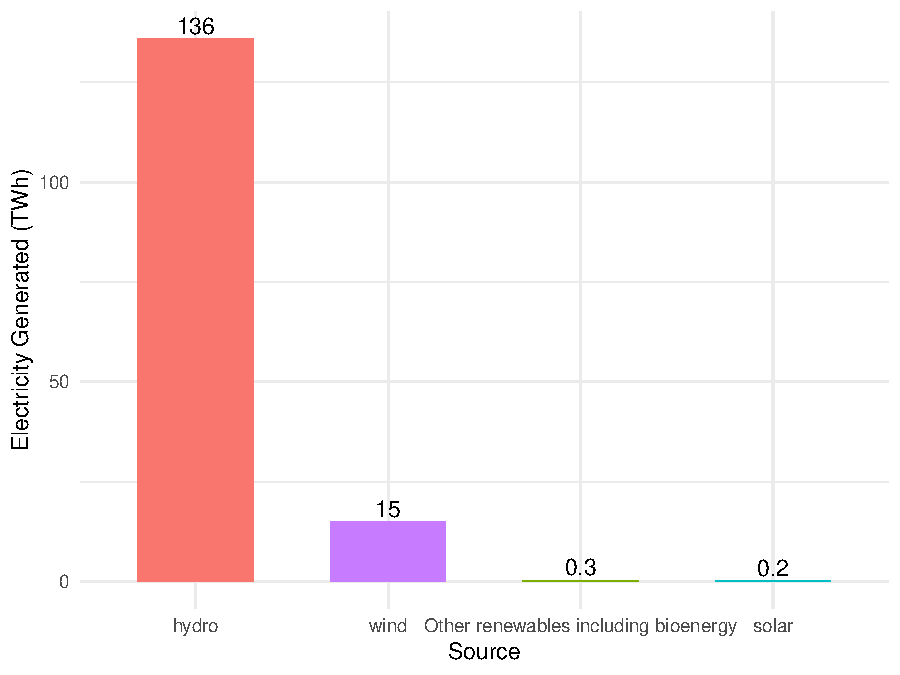
\includegraphics[keepaspectratio]{Assignment3_files/figure-pdf/fig-norway-sources-1.pdf}}

}

\end{figure}%

As shown in Table 2 and Figure 2, Norway's renewable electricity
generation in 2023 is overwhelmingly dominated by hydropower, which
accounts for approximately 136 TWh, making up more than 90\% of its
total renewable output. In comparison, wind energy contributed around 15
TWh, which is only about 10\% of the total. Both solar energy and other
renewables including bioenergy made negligible contributions, with
values of 0.17 TWh and 0.26 TWh, respectively.

This distribution highlights Norway's strong reliance on its abundant
hydrological resources, which are enabled by its mountainous terrain and
extensive water systems.

The limited output from wind and solar indicates that while Norway has
made some effort to diversify, its renewable success is not based on
technological breadth, but rather on natural geographic advantages.

This clear energy profile lays the foundation for further analysis in
the Results section, where we explore the historical, policy, and
environmental factors that have enabled Norway's exceptional performance
in renewable integration.

\subsection{Why Norway ranks highest globally in renewable energy
share?}\label{why-norway-ranks-highest-globally-in-renewable-energy-share}

To further explain why Norway ranks highest globally in renewable energy
share, we compare its energy source composition with that of other
top-performing countries. Figure 3 below compares total hydropower
generation in 2023 across selected countries. While China leads in
absolute hydropower output, Norway still ranks among the global top
producers despite its relatively small population and geographic size.

\begin{figure}

\caption{\label{fig-global-hydro}Global Hydropower Generation (TWh) in
2023 by Country}

\centering{

\pandocbounded{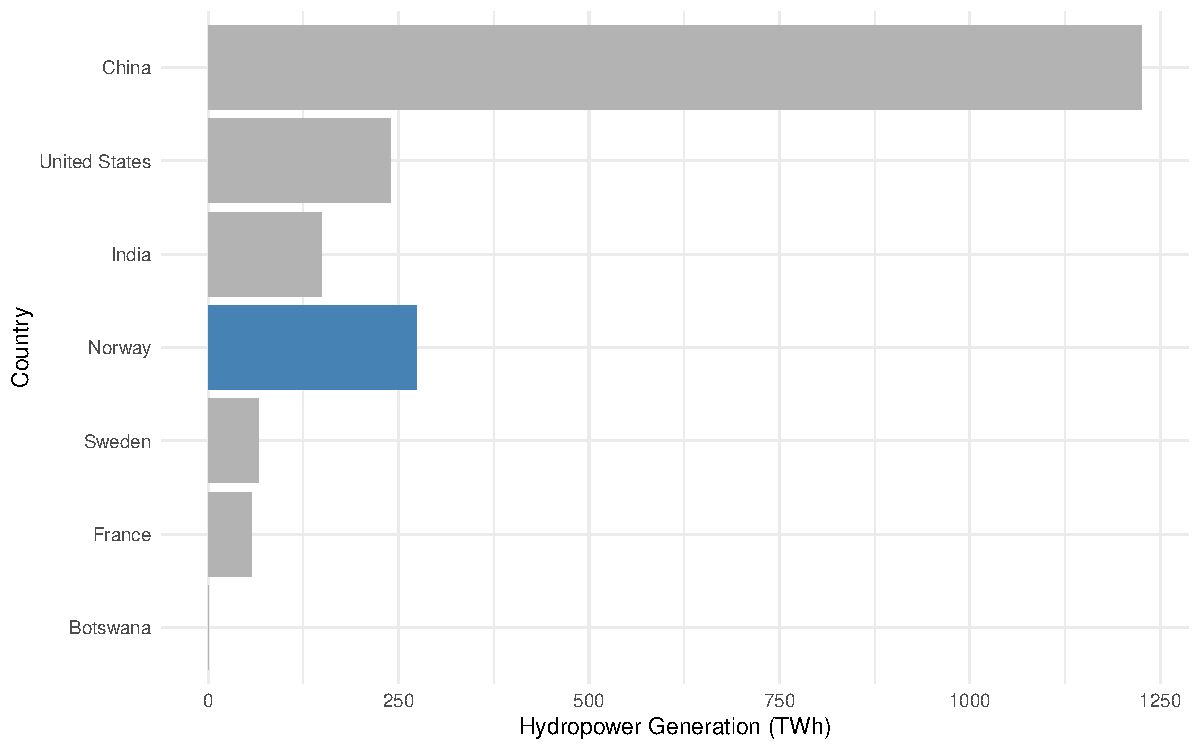
\includegraphics[keepaspectratio]{Assignment3_files/figure-pdf/fig-global-hydro-1.pdf}}

}

\end{figure}%

Figure 3 compares total hydropower generation in 2023 across
top-producing countries. While China leads with over 1,200 TWh, Norway
still ranks among the global top producers with approximately 270 TWh
--- despite its relatively small population and geographic size. This
reinforces the idea that Norway's dominance in renewable energy share is
not just a percentage artifact, but supported by substantial hydropower
infrastructure and generation capacity. Norway's natural topography has
enabled it to produce a significant amount of clean energy with low
variability.




\end{document}
